\chapter{Analysis of Smart Cafeteria}
\label{chap:AnalysisofSmartCafeteria}

In this chapter, I will explain the methodology
[\ref{sec:RequirementDataGathering}] and the result of analysis phase
[\ref{sec:DataAnalysis}] of ``Smart Cafeteria''. In the first section, I have
provided the definition of Requirements and Data Gathering techniques; and also
mentioned different data gathering techniques which were required to collect
requirements for ``Smart Cafeteria''. I have used some data gathering techniques
that are used to find and clarify the users' needs and requirements for ``Smart
Cafeteria''.


At the very beginning of analysis, I have started to study documents and
researched about ``Smart Cafeteria'' and found a set of stakeholders
[\ref{subsec:Stakeholders}], initial functional requirements [\ref{subsec:FR}]
and non functional requirements [\ref{subsec:NFR}].
Then I have studied Opera universitaria's documents related to Mensa and found a
few new requirements [\ref{subsec:MensaDocuments}]. To find out more
requirements for ``Smart Cafeteria'' I have made a focus group discussion
[\ref{subsec:FocusGroup}] and finally went through questionnaire
[\ref{subsec:Questionnaires}].


In the second section [\ref{sec:DataAnalysis}], I have presented data analysis and
result using previous set of requirements. The result was presented using UML
2.0 e.g. Use Case diagram [\ref{subsec:usecase}], Class Diagram
[\ref{subsec:classdiagram}] and Activity Diagram [\ref{subsec:activity}].


\section{Requirements and Data Gathering}
\label{sec:RequirementDataGathering}
\textbf{A Requirement} \cite{preece2002interaction} is a statement about a
proposed system that specifies what it should do or how it should perform it's
activities. One of the aim of the requirement activity is to make them as
specific, unambiguous, and clear as possible. Traditionally, there exists two
different kind of requirement; \textbf{functional requirements} which concerns
about what the system should do, and \textbf{non functional requirements} which
states about the constraints of the system and its development. The main reason
of the requirement analysis is to understand about the users, their work, and
the context , so that the system can be developed such a way which could satisfy
the requirements of the users. This is called identifying needs. On the other
hand, second aim is to produce a set of stable requirements that drive to next
phase which is design phase.
Identifying needs and establishing requirements is itself an iterative activity
in which the sub activities inform and refine one another. It does not last for
a precise number of weeks or months, it lasts until it achieves usability goals.

The purpose of \textbf{data gathering} is to find  a set of stable requirements
even though a set of initial requirement exists, data accumulation will help to
expand, clarify, and confirm those initial requirements. Data accumulation needs
to cover a wide spectrum of issues because the different kind of requirements
needed to be established~\cite{preece2002interaction}.

There are very few number of basic techniques to gather data, but they are very
important and flexible which could be combined and extended in many ways.
These will give scope to understand the  variety of requirements and these
techniques are commonly studying documentation, questionnaires, interviews,
focus groups and workshops, users' observation.

\subsection{Stakeholders}
\label{subsec:Stakeholders}
Stakeholders are the people from whom all requirements will be gathered, the
people who has the most influence on design and the people who will get 
benefited from the completed project. Here is the list of all stakeholders of the
smart cafeteria.
\begin{enumerate}
\item \textbf{System Users:} System user is those who are going to use and get
services from our system ``smart cafeteria''. They are usually students,
professors, researchers, University administration officers and University
technical staffs who are closely involved with our system. Their main goal is to
search food menu in online system application and order menu through online to
reduce mensa queue time.
\item \textbf{Students:} Students are one of the most important stakeholder who
belongs to system users. Basically most of the students are busy with their
classes, examinations and they stay at the university almost entire day and
generally take their breakfast, lunch and some cases even their dinner in
cafeteria.
\item \textbf{Professors:} Professors are one of the most important stakeholder
who will be system users. They are mostly busy with their classes, seminars,
projects in all day long at the university.
\item \textbf{Researchers:} Researchers are another kind of stakeholder and
system users who are going to use this system to get services.
\item \textbf{Administrative Officer \& Technical Staff:} University
administrative officers \& technical staffs are system users and stakeholder.
They stays busy with their work all day long and also take their lunch at
university cafeteria. So they will also get services and facilities from this
system.
% \item \textbf{University's Technical Staff:} University's technical staffs are
% system users and also will be one stakeholder of this system.
\item \textbf{System Administrator:} System administrator is a kind of
stakeholder of this system who is going to manage the system, update menu in the
system, check the order and add all kind of information related to cafeteria in
the system. Cafeteria staffs are the mainly system administrator and their main
goal is to spread food menu information through online.
\item \textbf{Cafeteria Staff:} They are one kind of stakeholder and a
kind of system administrator who is going to check the order and serve the menu
for the other stakeholders.
\end{enumerate}

\subsection{Initial Functional Requirements}
\label{subsec:FR}
As a cafeteria user I have done initial analysis and found some initial
functional requirements from my previous experience and knowledge  which is
discussed in this section. To find out more requirements and make the system
stable, I have studied cafeteria's food menu and related documents
[\ref{subsec:MensaDocuments}], built focus group [\ref{subsec:FocusGroup}] and
conducted interview with questionnaires [\ref{subsec:Questionnaires}].

In software engineering, a functional requirement defines the functions of a
software system and its component \cite{Karthika2012}. A function is described
as a set of input, it's behavior, and outputs. Functional requirements may be
calculations, technical details, data manipulation, processing and other
specific functionality that describes what a system will do. The system uses the
functional requirements that are captured in use cases. All functional
requirements are supported by non functional requirements which impose some
constraints  such as security, reliability, portability on the design and
implementation of the system. Functional requirement catches the proposed
behavior as services, tasks or functions of the system that is required to
achieve goals.

The functional requirements of ``Smart Cafeteria'' as follows which is
categorized by different roles and tasks in the application.
\begin{enumerate}[(I)]
\item \textbf{System Users:} System users have the principle role in the system
application. They are basically students, professors, researchers, university
administration officers and university technical staffs who are going to use the
system. After research, I have found the following functionalities of the system
users into the ``Smart Cafeteria'' which has been shown in table
\ref{tab:FRSystemUsers}.

\begin{table}[h!t]
\centering
%\captionof{table}{Usefulness} \label{tab:Usefulness} 
 \begin{tabular}{| p{2cm} | p{10cm} |}
    \hline
    Serial No. & Functional Requirements \\ \hline
    F1 & User should register in the system to get services. \\ \hline
    F2 & Registration confirmation through email. \\ \hline
    F3 & Forgot user name or password. \\ \hline
    F4 & Login into the system. \\ \hline 
  	F5 & Login into system through application login function. \\ \hline 
    F6 & Login into system through university's login service. \\ \hline 
    F7 & Check users own dashboard after login. \\ \hline 
 	F8 & User can update user's own information and credential (change profile information, password). \\ \hline
 	F9 & follow users. \\ \hline 
 	F10 & view User's activities. \\ \hline 
 	F11 & View list of food menu. \\ \hline 
 	F12 & Search food menu. \\ \hline 
 	F13 & View menu details. \\ \hline 
 	F14 & Place oder menu. \\ \hline 
  	F15 & Payment for order. \\ \hline 
   	F16 & View order statistics. \\ \hline
   	F17 & View dieting report and calorie consumption per day. \\ \hline
   	F18 & Generate dieting report. \\ \hline
   	F19 & Rating in food menu . \\ \hline
   	F20 & Give comments in individual food menu. \\ \hline
   	F21 & Generate report. \\ \hline 
   	F22 & Take food menu receipt after placing order by punching student card into the POS terminal. \\ \hline 
    \end{tabular}
 \caption{Functional Requirements of System Users.}
\label{tab:FRSystemUsers}
\end{table}

\item \textbf{System Administrator:} System administrators who are basically
cafeteria's staffs have the following functionalities that has been shown in the
table \ref{tab:FRSystemAdministrator}.

\begin{table}[h!t]
\centering
%\captionof{table}{Usefulness} \label{tab:Usefulness} 
 \begin{tabular}{| p{2cm} | p{10cm} |}
    \hline
    Serial No. & Functional Requirements \\ \hline
    F23 & Login in admin panel. \\ \hline
    F24 & Add food menu in the system. \\ \hline
    F25 & Edit food menu. \\ \hline
    F26 & Delete food menu. \\ \hline 
  	F27 & Manage order. \\ \hline 
    F28 & View order. \\ \hline 
    F29 & View order statistic per day (Total order). \\ \hline 
 	F30 & View order statistic per week. \\ \hline
 	F31 & View order statistic by menu. \\ \hline 
 	F32 & view User's activities. \\ \hline 
  	F33 & Search order by food menu. \\ \hline
  	F34 & Search food menu by name and key word. \\ \hline 
  	F35 & Generate report. \\ \hline 
    \end{tabular}
 \caption{Functional Requirements of System Administrator.}
\label{tab:FRSystemAdministrator}
\end{table}

\item \textbf{System Application:} System application itself has some
functionality which has to be performed to make the system more interactive. The
functionalities of system application has been shown in table
\ref{tab:FRSystemApplication}.

\begin{table}[h!t]
\centering
%\captionof{table}{Usefulness} \label{tab:Usefulness} 
 \begin{tabular}{| p{2cm} | p{10cm} |}
    \hline
    Serial No. & Functional Requirements \\ \hline
    F36 & Generate daily food menu notification through email or sms. \\ \hline
    F37 & Generate weekly food menu notification to users. \\ \hline
    F38 & Suggesting list of food menu to users based on their choice rating and
which food menu they have took daily and how much calorie they have took in the last
couple of weeks. \\ \hline
    F39 &  Order status will be kept pending until user takes the receipt from POS
terminal. \\ \hline 
  	F40 & Order status confirm after users take food menu receipts by punching
student card. \\ \hline 
    \end{tabular}
 \caption{Functional Requirements of System Application.}
\label{tab:FRSystemApplication}
\end{table}

\item \textbf{POS Terminal:} POS terminal is used for payment through master
card in most of shops or supper market. But in ``Smart cafeteria'' it could be
used to pay or print order receipt after order food and successfully paying
online. The POS terminal has some functionalities which has shown in the table
\ref{tab:FRPOSTerminal}.

\begin{table}[h!t]
\centering
%\captionof{table}{Usefulness} \label{tab:Usefulness} 
 \begin{tabular}{| p{2cm} | p{10cm} |}
    \hline
    Serial No. & Functional Requirements \\ \hline
    F41 & Print food menu order receipt after punching card into the POS terminal machine. \\ \hline
    F42 & Send a notification to the system that user got the receipt after order. \\ \hline
       \end{tabular}
 \caption{Functional Requirements of POS Terminal.}
\label{tab:FRPOSTerminal}
\end{table}
\end{enumerate}

\subsection{Non Functional Requirements}
\label{subsec:NFR}
Non functional requirement defines sometimes as system qualities and properties
of the system such as performance, security, maintainability in order to support
functional requirements. In other words, how well some behavioral or structural
view of the system could be accomplished.
The ``IEEE-Std 830 - 1998"\footnote{ IEEE Std 830-1998, Recommended Practice for
Software Requirements Specifications IEEE Recommended Practice for Software
Requirements Specifications} has discussed some non-functional
requirements~\cite{Committee1998} in a Software Requirements Specification and
after research, I have found the following non functional requirements for
``Smart Cafeteria'':
% \begin{itemize}

\renewcommand{\labelenumi}{\arabic{enumi}.}
\renewcommand{\labelenumii}{(\roman{enumii})}


\begin{enumerate}

\item \textbf{Usability:} Usability is the most important non functional
requirement in smart cafeteria project and our main focus is on system usability
from non functional requirements along with the functional requirements of the
system. Usability is the activities with which a user can learn to operate,
easily understand inputs for and outputs of the system or component. From
previous discussion \ref{sec:HeuristicsUsability}, usability is generally
regarded as ensuring that interactive systems are effective to use, easy to
learn and enjoyable from user's perspective. Our system should also hold the
usability heuristics principles which is discussed earlier.

\item \textbf{Internationalization:} Since students in the University of Trento
are from various cultures and speakes different languages, our proposed system
should support multi language interfaces and functionalities.

\item \textbf{Portability:} The proposed system will be portable since the
system application will be accesable from Desktop PC, Laptop, Tablet as well as
Smart phone. This application will definitely support the non functional
requirement ``portability''.

\item \textbf{Adaptability:} According to \citet{Subramanian2001}, adaptation of
software systems is an unavoidable process which needs faster development of new
 or maintenance of existing software systems  due to the change in customer
requirements. There are also several definitions of adaptability which are taken
from several papers; some of those definitions are described bellow:
\begin{enumerate}
\item  According to ~\citet{Oreizy:769885:Gorlick}, ``Self-adaptive software
modifies its own behavior in response to changes in its operating environment''.

\item  ``Adaptability is defined as the ease with which a system or parts of the
system may be adapted to the changing
requirements~\cite{Subramanian2001,Tekinerdogan}.''

\item  ``A program is called adaptable if it can be easily changed. A program is
called adaptive if it changes its behavior automatically according to its
context~\cite{Subramanian2001,Lieberherr1995}".
\end{enumerate}
There are several things of software adaptation in our proposed smart cafeteria
system and one of them is the system capable of accepting http/https request
from different clients such as desktop, tablet as well as different versions OS
of smart phone and respond to them as well.


\item \textbf{Safety and security:} Safety and security is heighly important
non functional requirements of a system. There are some safety
and security non functional requirements propose in our smart campus
project and those are as follows:
\begin{enumerate}
\item  Our proposed system ensures authorized access to the system data as well as
user information.
\item The communication between the application server and client must be
encrypted and use https protocol.
\item Backup of all the system data should be taken every 24 hours and it should
be saved in a secure location.
\item System makes sure to stop if there is a any probability of security attacks.
\end{enumerate}

\item \textbf{Reliability:} In the software requirements specification
(SRS)\footnote{ IEEE Std 830-1998, Recommended Practice for Software
Requirements Specifications.}, Reliability is the most common non functional
requirement. There are some proposed non functional requirement for reliability in
our smart campus project and those are as follows:
\begin{enumerate}
\item	System should be available 24 hours.
\item	System should not have any failure during operation.
\item	Good reputation towards user.
\item	Deliver such services and functionalities that user can trust.
\end{enumerate}
\item \textbf{Performance:} Performance is a common non functional
requirement for a system. The following things should be available in our
system as non functional requirements:
\begin{enumerate}
\item Speed should be good in the operation of the system.
\item Response time of the operation should be good in any platform e.g. in
desktop, tablet, smart phone.
\end{enumerate}

\item \textbf{Documentation Requirements:} According to Software Requirement
Specification, ``Smart Cafeteria'' will specify and maintain proper
documentation before the start of development. The document should contain Title
and Author, scope, stakeholder, functional requirements, usability requirements,
technical requirements accordingly IEEE Std.

\end{enumerate}


\subsection{Studying Cafeteria's Food Menu and Documents}
\label{subsec:MensaDocuments}
Studying documentation is an important part of data gathering technique.
Procedures and rules are written down sometimes in manuals or papers and these
are a good source of data. In the requirement activity, studying documentation
is good for understanding legislation and getting some background information
about the work as well as the system~\cite{preece2002interaction}. Since
studying documents is essential, I have researched and studied about Mensa's
food menu [ Figure \ref{fig:differentmenu}] and Mensa's other documents
[Appendix~\ref{sec:MenuAppendix}] of Opera Universitaria di
Trento~\cite{operauniversity}(university of Trento).
\begin{figure}[h!t]
    \centering
      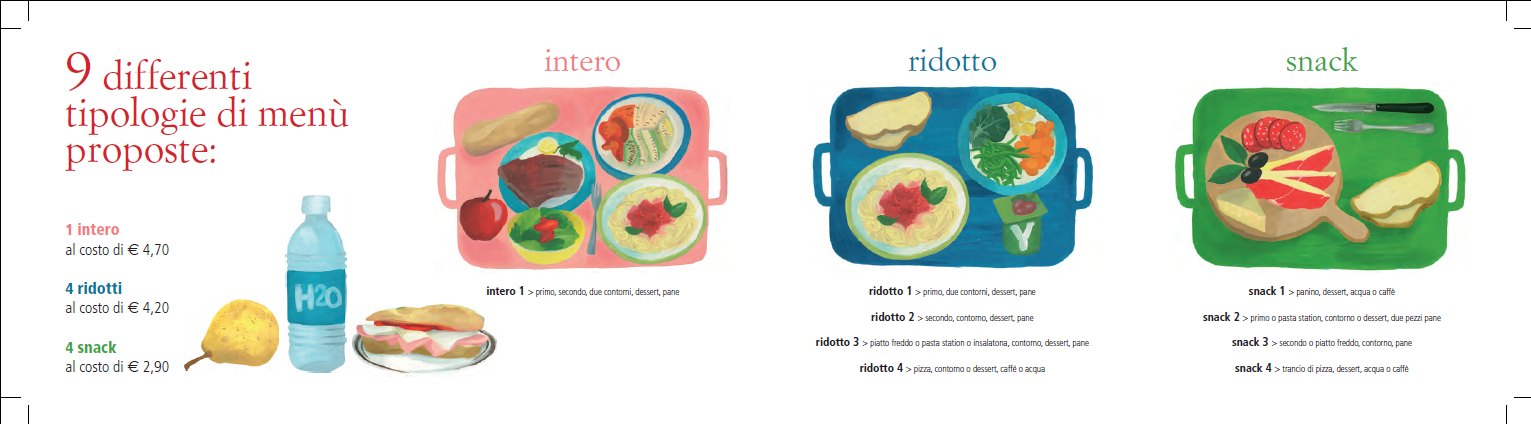
\includegraphics[width=5.5in,height=2in]{ch3/AppendixMenu/differentmenu}
  \caption{different menu of Mensa in University of Trento.}
  \label{fig:differentmenu}
\end{figure}
From this research, I have found the following facts:
\begin{itemize}
\item Since university of Trento has several departments in the several places,
university has a lot of cafeteria branch in different place as well.
\item I have also found that all cafeteria branches have a monthly opening time
schedule in the website as a pdf document.
\item I have also found each cafeteria offers different food menu such as full
menu, reduce menu and snack charging of different prices and where each menu contains
different food items and calories as well.
\end{itemize}
From those of facts, I have come down into a decision and added some more
functional requirements into the system. The additional functional requirements
as follows:\\ \\
\textbf{System administrator}
\begin{enumerate}
\item System administrator can add, edit and delete operation into the
system for cafeteria branch.
\item System administrator can add, edit and delete monthly operating time
schedule of each branch into the system; for example, povo1 is closed January 1
to January 6, 2013 and others working days of the month January 2013 will be
opened.
\item System administrator can add, edit and delete food item which contains
food item status e.g. first course, second course, dessert, side dishes, cold
drinks, etc. and their respective Kilo calories per 100gm and other
information's.
\end{enumerate}
\textbf{System users}
\begin{enumerate}
\item System users can see and browse the cafeteria branches and monthly
operating time schedule of each branch respectively.
\item System user can create own menu using menu wizard from different food
items depending on their choice which may have different cost depending on food
items.
\end{enumerate}

\subsection{Focus Group}
\label{subsec:FocusGroup}
Focus group and workshop is a very good technique to gather data and set of
requirements. Interview is a such kind of thing which tends to be one on one
perspective where as focus group and workshop is a very effective, alternative
and collaborative technique to get a group of stakeholders together to discuss
about the system and find out set of requirements. This activity sessions should
be very structured with predefined set topics for discussion and I was as a
facilitator in that focus group session and I have discussed and asked several
questions[Appendix~\ref{sec:DataGatheringQuestionnaire}] about our smart
cafeteria system and its facilities and functionalities.
The participants took part in open discussions as well as gave answers to the
questionnaires \cite{preece2002interaction}.

There were 7 participants in this session, all of them are the student of
University of Trento who used to take their lunch in University's cafeteria.
In the Table \ref{tab:FocusGroup} [Appendix~\ref{sec:AppendixFocusGroup}] , the
summary of the focus group meeting are shown.

\begin{table}[h!t]
\centering
%\captionof{table}{Usefulness} \label{tab:Usefulness} 
 \begin{tabular}{| p{3cm} | p{4.5cm} | p{4.5cm} |}
    \hline
    Agenda Item & Discussion &  Decision\\ \hline
    
    Smart Cafeteria Functional Requirements & We discussed all functional
    requirements that I have found earlier. & They agree with all functional
    requirements and they suggested one extra functional requirements which is
    mobile application should support QR BARCODE. \\ \hline
    
    Smart Cafeteria Non Functional Requirements & We have discussed all non
    functional requirements from IEEE-Std 830 - 1993'.& All participants strongly
    supported Internationalization, Usability and Portability.\\ \hline
   
    Smart Cafeteria in mobile and Tablet apps & Now we are in the age of
    informational technology, especially in mobile computing phase where all
    applications drive to support in mobile and tablet in smartly. & All
    participants strongly supported smart cafeteria mobile applications.\\ \hline
    
    Adaptive mobile application & Adaptive application will observe user
    behavior, test, and user's psychology and conclude a result with the help of
    machine learning techniques and finally suggests a list of solutions. & All
    participants strongly supported smart cafeteria mobile applications which
    must be adaptive application.\\ \hline
       \end{tabular}
 \caption{Focus Group Discussion Summary.}
\label{tab:FocusGroup}
\end{table}

From the discussion, I have found requirements that, since the application also
supports mobile plateform, so the application could scan QR BARCODE
[Figure-~\ref{QRBARCODE}] which along with food menu automatically it forces to
order menu phase. In the [Appendix~\ref{sec:DataGatheringQuestionnaire}], the
questions asked to participants is shown.

\begin{figure}[h!t]
    \centering
      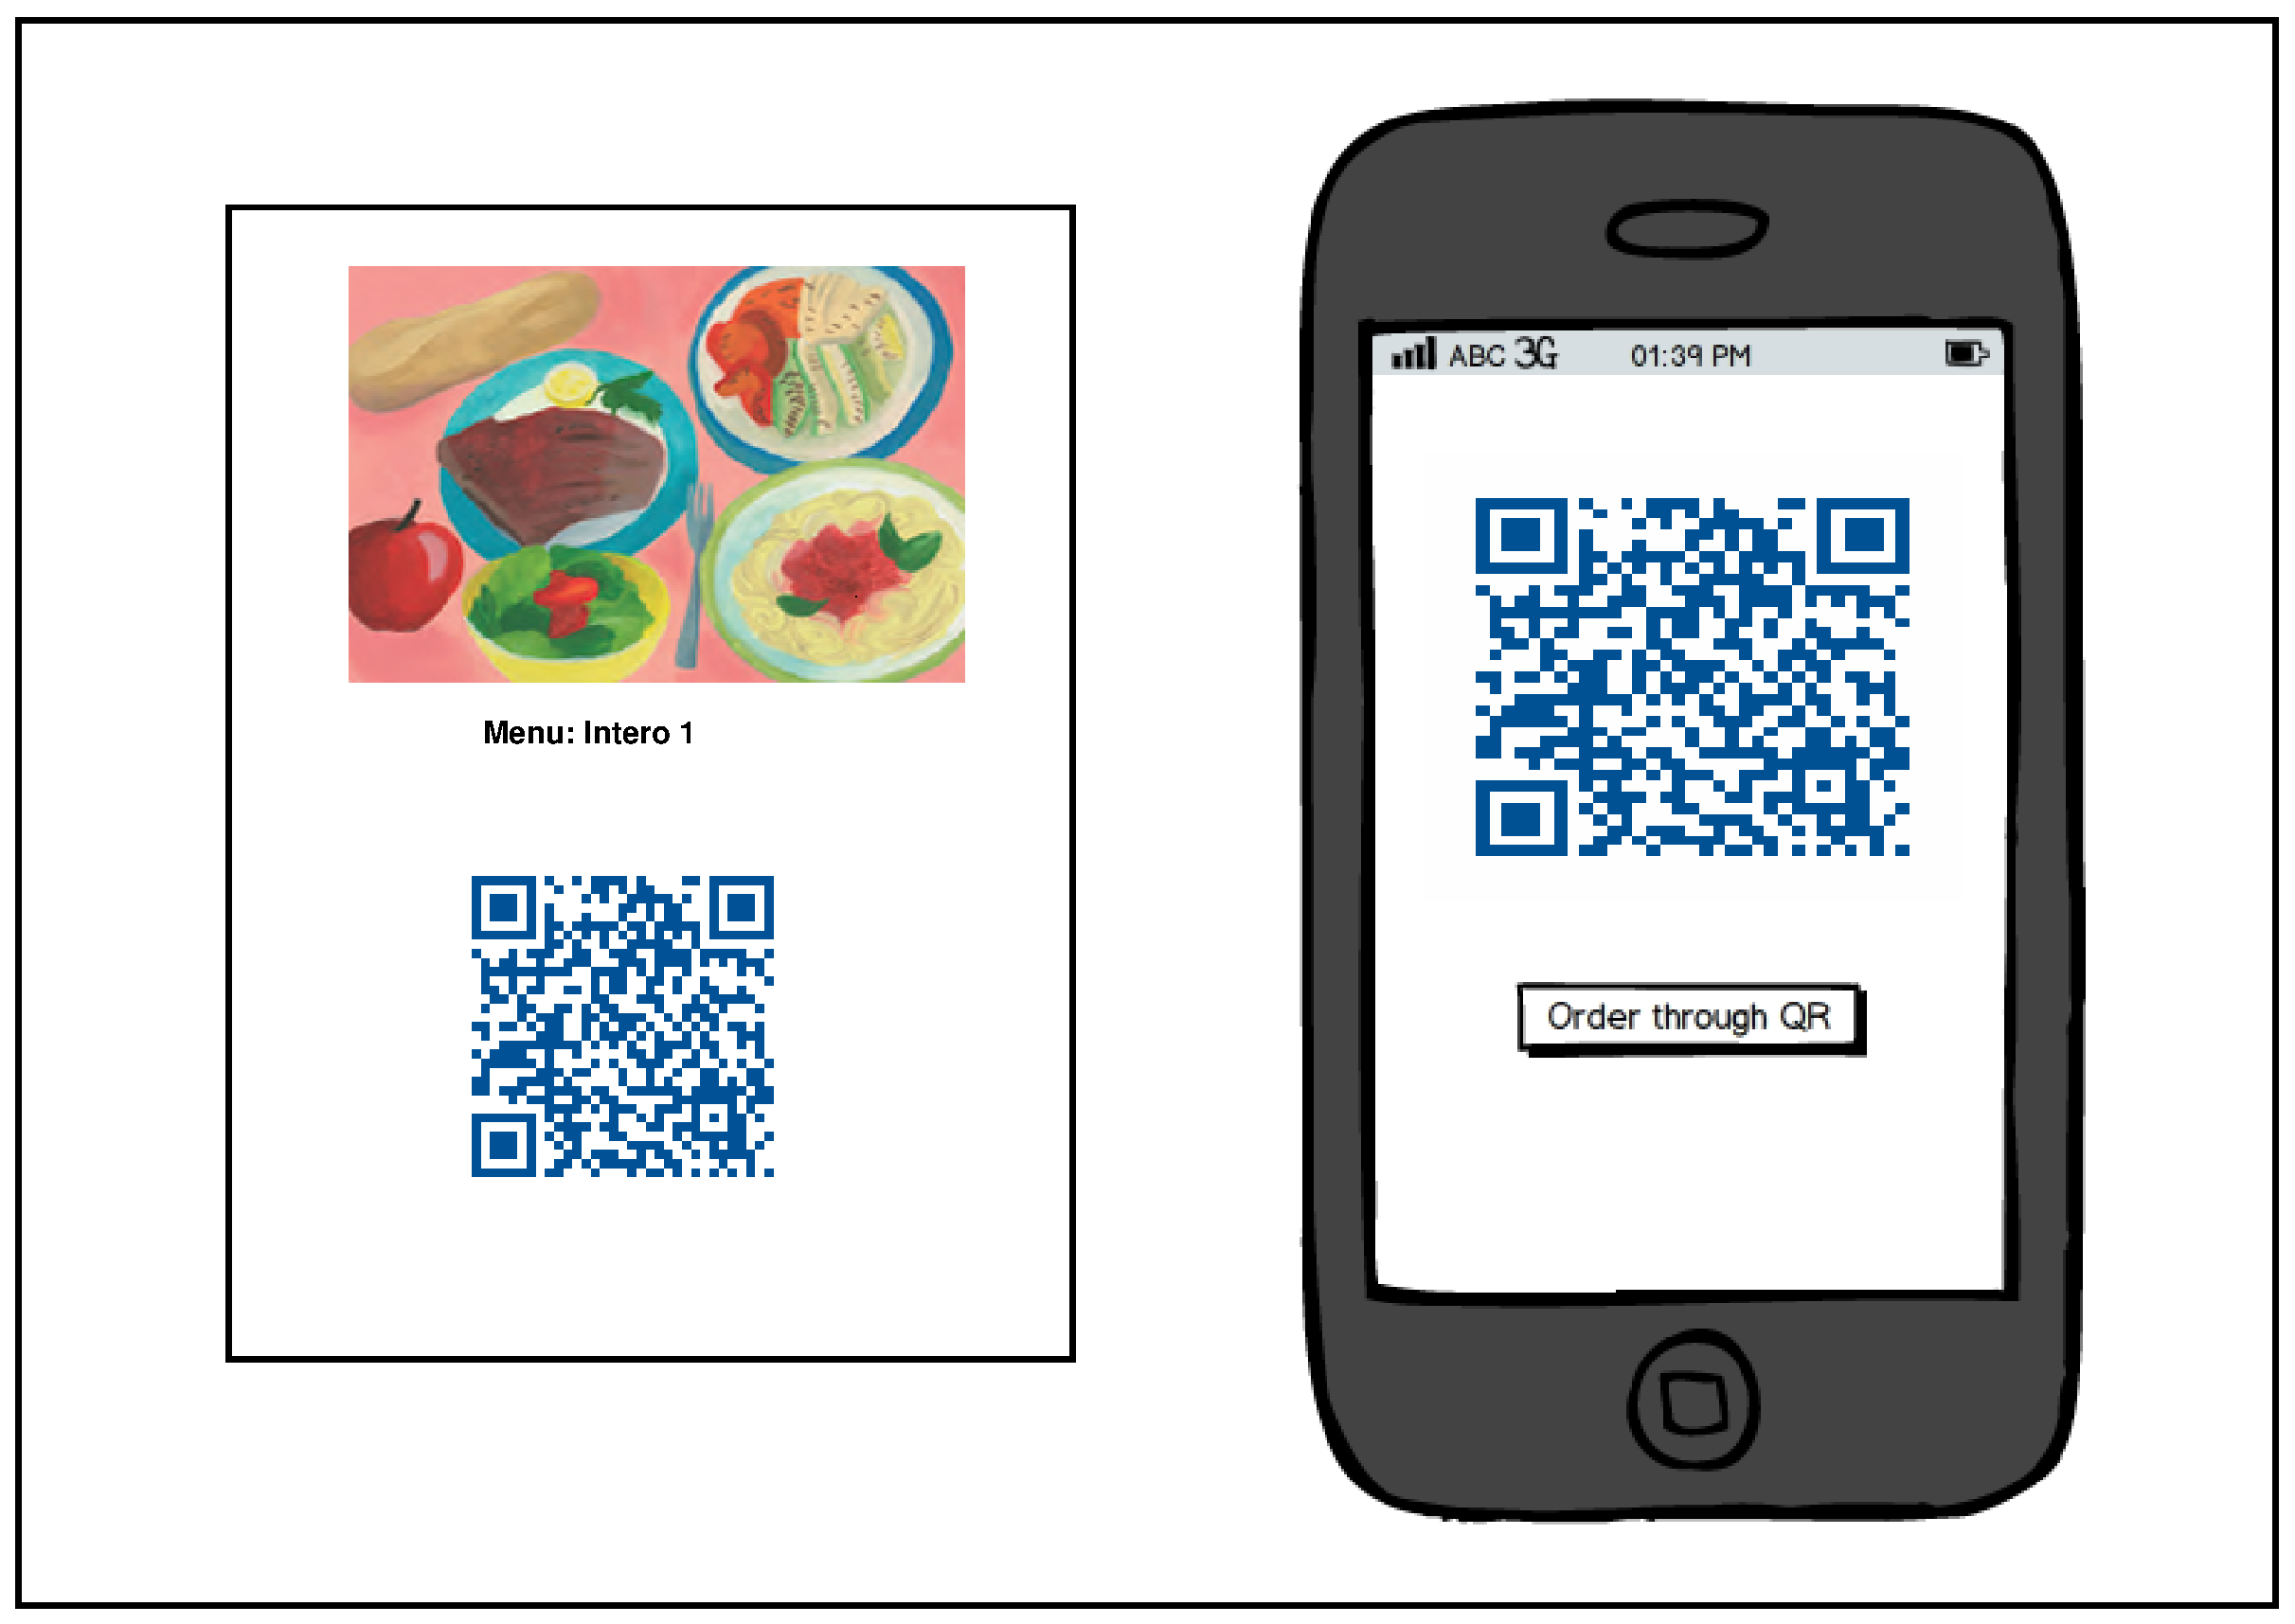
\includegraphics[width=5.5in]{ch3/FocusGroup/QRBARCODE}
  \caption{QR BARCODE}
  \label{QRBARCODE}
\end{figure}

\subsection{Questionnaires}
\label{subsec:Questionnaires}
\citet{AdamsAnneandCox2008} have defined that Questionnaires are usually paper
based or delivered online and consist of a set of questions which all
participants are asked to complete. Questionnaire is a kind tool that should be
easily understandable, interpretable; and should avoid complex words.
Questionnaires should hold reliability and validity; to increase the
effectiveness of questionnaires it is important that how it is structured and
it's unambiguity. Questionnaires should preserve interviewers' trust, privacy
and ethics; so interviewer should ensure confidentiality.
They also found that if a large number of users are participating, there
always have a chance to get a large amount of data which need to be coded and
analysed. They also suggested that focus group is better than conducting
single interview since interviews are usually conducted on a one-to-one basis.
It requires a large amount of the investigator's time during the interviews as
well as  transcribing and analyzing the data.

There were seven questions whose scale was based upon the Likert scale Effective
or not Effective and yes or no. On the other hand, two questions were for open
suggestions to improve the system's functionalities. The Table
\ref{tab:DataGatheringQuestionnaire}
[Appendix~\ref{sec:DataGatheringQuestionnaire}] has shown the questionnaire
which have asked to participants in focus group meeting and the number of
participants agreed or disagreed with the facts from total 7 participants.

\begin{table}[h!t]
\centering
%\captionof{table}{Usefulness} \label{tab:Usefulness} 
 \begin{tabular}{| p{8.5cm} | p{2cm} | p{2cm} |}
    \hline
    Questions/Answer & Yes or Effective &  No or Not Effective\\ \hline
    
    Do you support if an application which will provide mensa system where avoiding
    a long queues and saving time? & 7  & 0 \\ \hline
    
    If there will be an application where you could browse food menu, search
    food menu, order and pay online, then how effective the system will be ? & 7
     & 0 \\ \hline
    
    If the application let you create your own food menu as real
    scenario, how effective the system will be for you? & 5 & 2 \\ \hline
    
    how effective the system will be if the application supports mobile
    plateform? & 6 & 1 \\ \hline
    
    If the application could suggest you food menu depending on your choice,
    test, your dieting preferences, then how effective the system will be?  &
    7 & 0 \\ \hline
    
    If the application provides support in different languages, then how
    effective the system will be? & 7 & 0 \\ \hline
    
	Do you think that this application may help you or make your university life
	easier?  & 6 & 1 \\ \hline	

\end{tabular}
 \caption{Data Gathering Questionnaire \& Result.}
\label{tab:DataGatheringQuestionnaire}
\end{table}


\section{Data Analysis}
\label{sec:DataAnalysis}
Data interpretation and analysis is a very important part in the interactive
system development life-cycle. When Data-gathering session has been almost
finished, data interpretation and analysis phase could start and it is an
iterative step between data gathering and data analysis.

In data analysis~\cite{preece2002interaction}, different techniques and
notations were followed to find different aspects of the system that will give
different requirements. Traditionally, functional requirements have been
analyzed and expressed using data-flow diagrams, state charts diagram, work-flow
charts. Since our system development is using object-oriented approach,
functional and data requirements are combined in class diagrams and behavior of
the system being expressed using sequence diagrams. Use case focuses on goals of
users which were introduced through the object-oriented community . Use case
focuses specifically on the interaction between the user and a software system.
The term scenario is also used in the context of use cases.

In the following Subsections~\ref{subsec:usecase},~\ref{subsec:classdiagram}
and~\ref{subsec:activity} , I will describe and discuss about Use case diagrams,
Class diagram and Activity diagrams of ``Smart Cafeteria'' respectively.

\subsection{Use Case Diagram}
%\phantomsection
\label{subsec:usecase}
According to UML 2.0  specification~\cite{UML:2007:Specification}, a use case
diagram represents the relationship between actors and use cases within a
system. The use cases represent functionality of a system or a classifier as
like a subsystem or a class, as manifested to external integrator with the
system or the classifier. A use case diagram contains a set of actors, set of
use cases, some interfaces; and shows the relationships between these elements.
The relationships are mainly associations between the actors and the use cases;
generalizations, extend and includes among use cases; and generalizations
between the actors.

Since I have discovered some stakeholders and their goals in this system after
analysis, depending on those I have found four use cases scenarios. Bellow I
will describe those use case scenario one by one.

\subsubsection{Use case of System users}

In this use case, students, professors, researchers, university staffs all are
generalized as system user basically who are going to use the system to get some
service from ``Smart Cafeteria'' system.
System user can perform basic operation like registration, confirm registration,
forgot password, login and logout. Login could be performed through university's
authentication service and its own application login. After login into the
system users could access their own dashboard from where they could perform
search food menu, view list of food menu, view individual food menu, rating in
food menu, comments on food menu, place order food menu, change user's profile,
view dieting report. Through this system, users could also make their own food
menu using create menu wizard. System user could also see information about
cafeteria branches and their time schedule through the system. After order and
payments, system users must take a menu receipt after punching their card in the
POS terminal.

\begin{landscape}
\begin{figure}[h!t]
    \centering
    \fbox{
      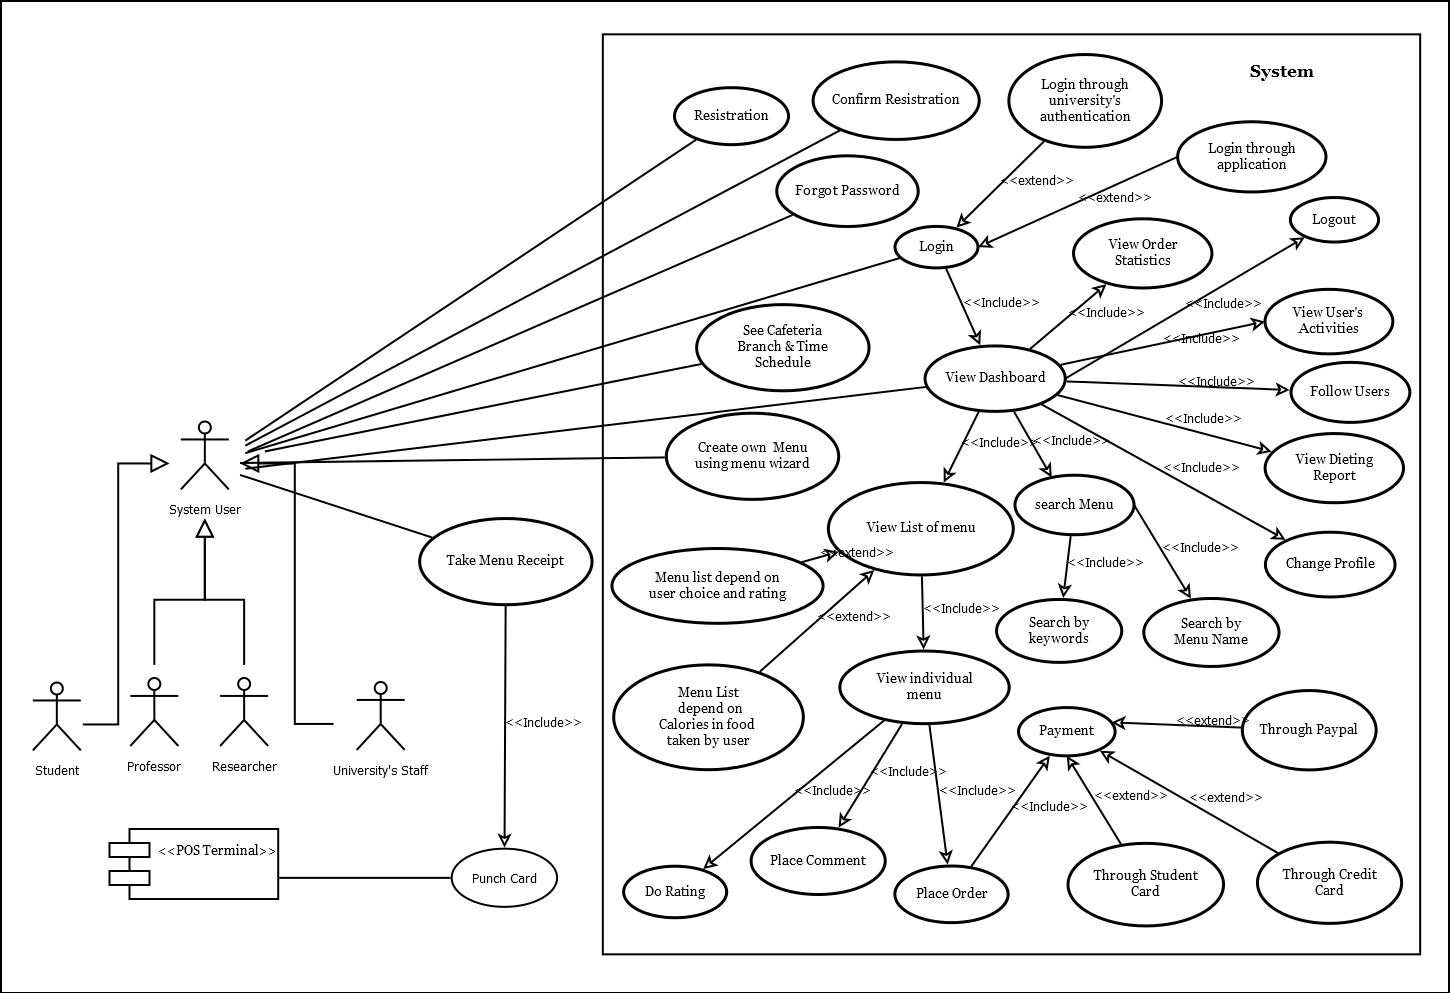
\includegraphics[width=8in]{ch3/UseCase/SystemUser}
      }
  \caption{Use Case Diagram of System User}
  \label{UCSystemUser}
\end{figure}
\end{landscape}

\subsubsection{Use case of System Administrator}

In the use case of system administrator, cafeteria staff's are generalized as
system administrator.
System administrator can perform their operation after login into the system.
After login, system administrator can access administrator dashboard. And from
administrator dashboard, system administrator can manage cafeteria branch which
means add, edit, delete and view operation on cafeteria branch and their
respected time schedule. System administrator can add, edit, delete and view
operation on food item and menu.
They also can make food menu from food item and menu. System user can view order
statistics, view total order, view order pending, generate various kind of
report.
\begin{landscape}
\begin{figure}[h!t]
    \centering
      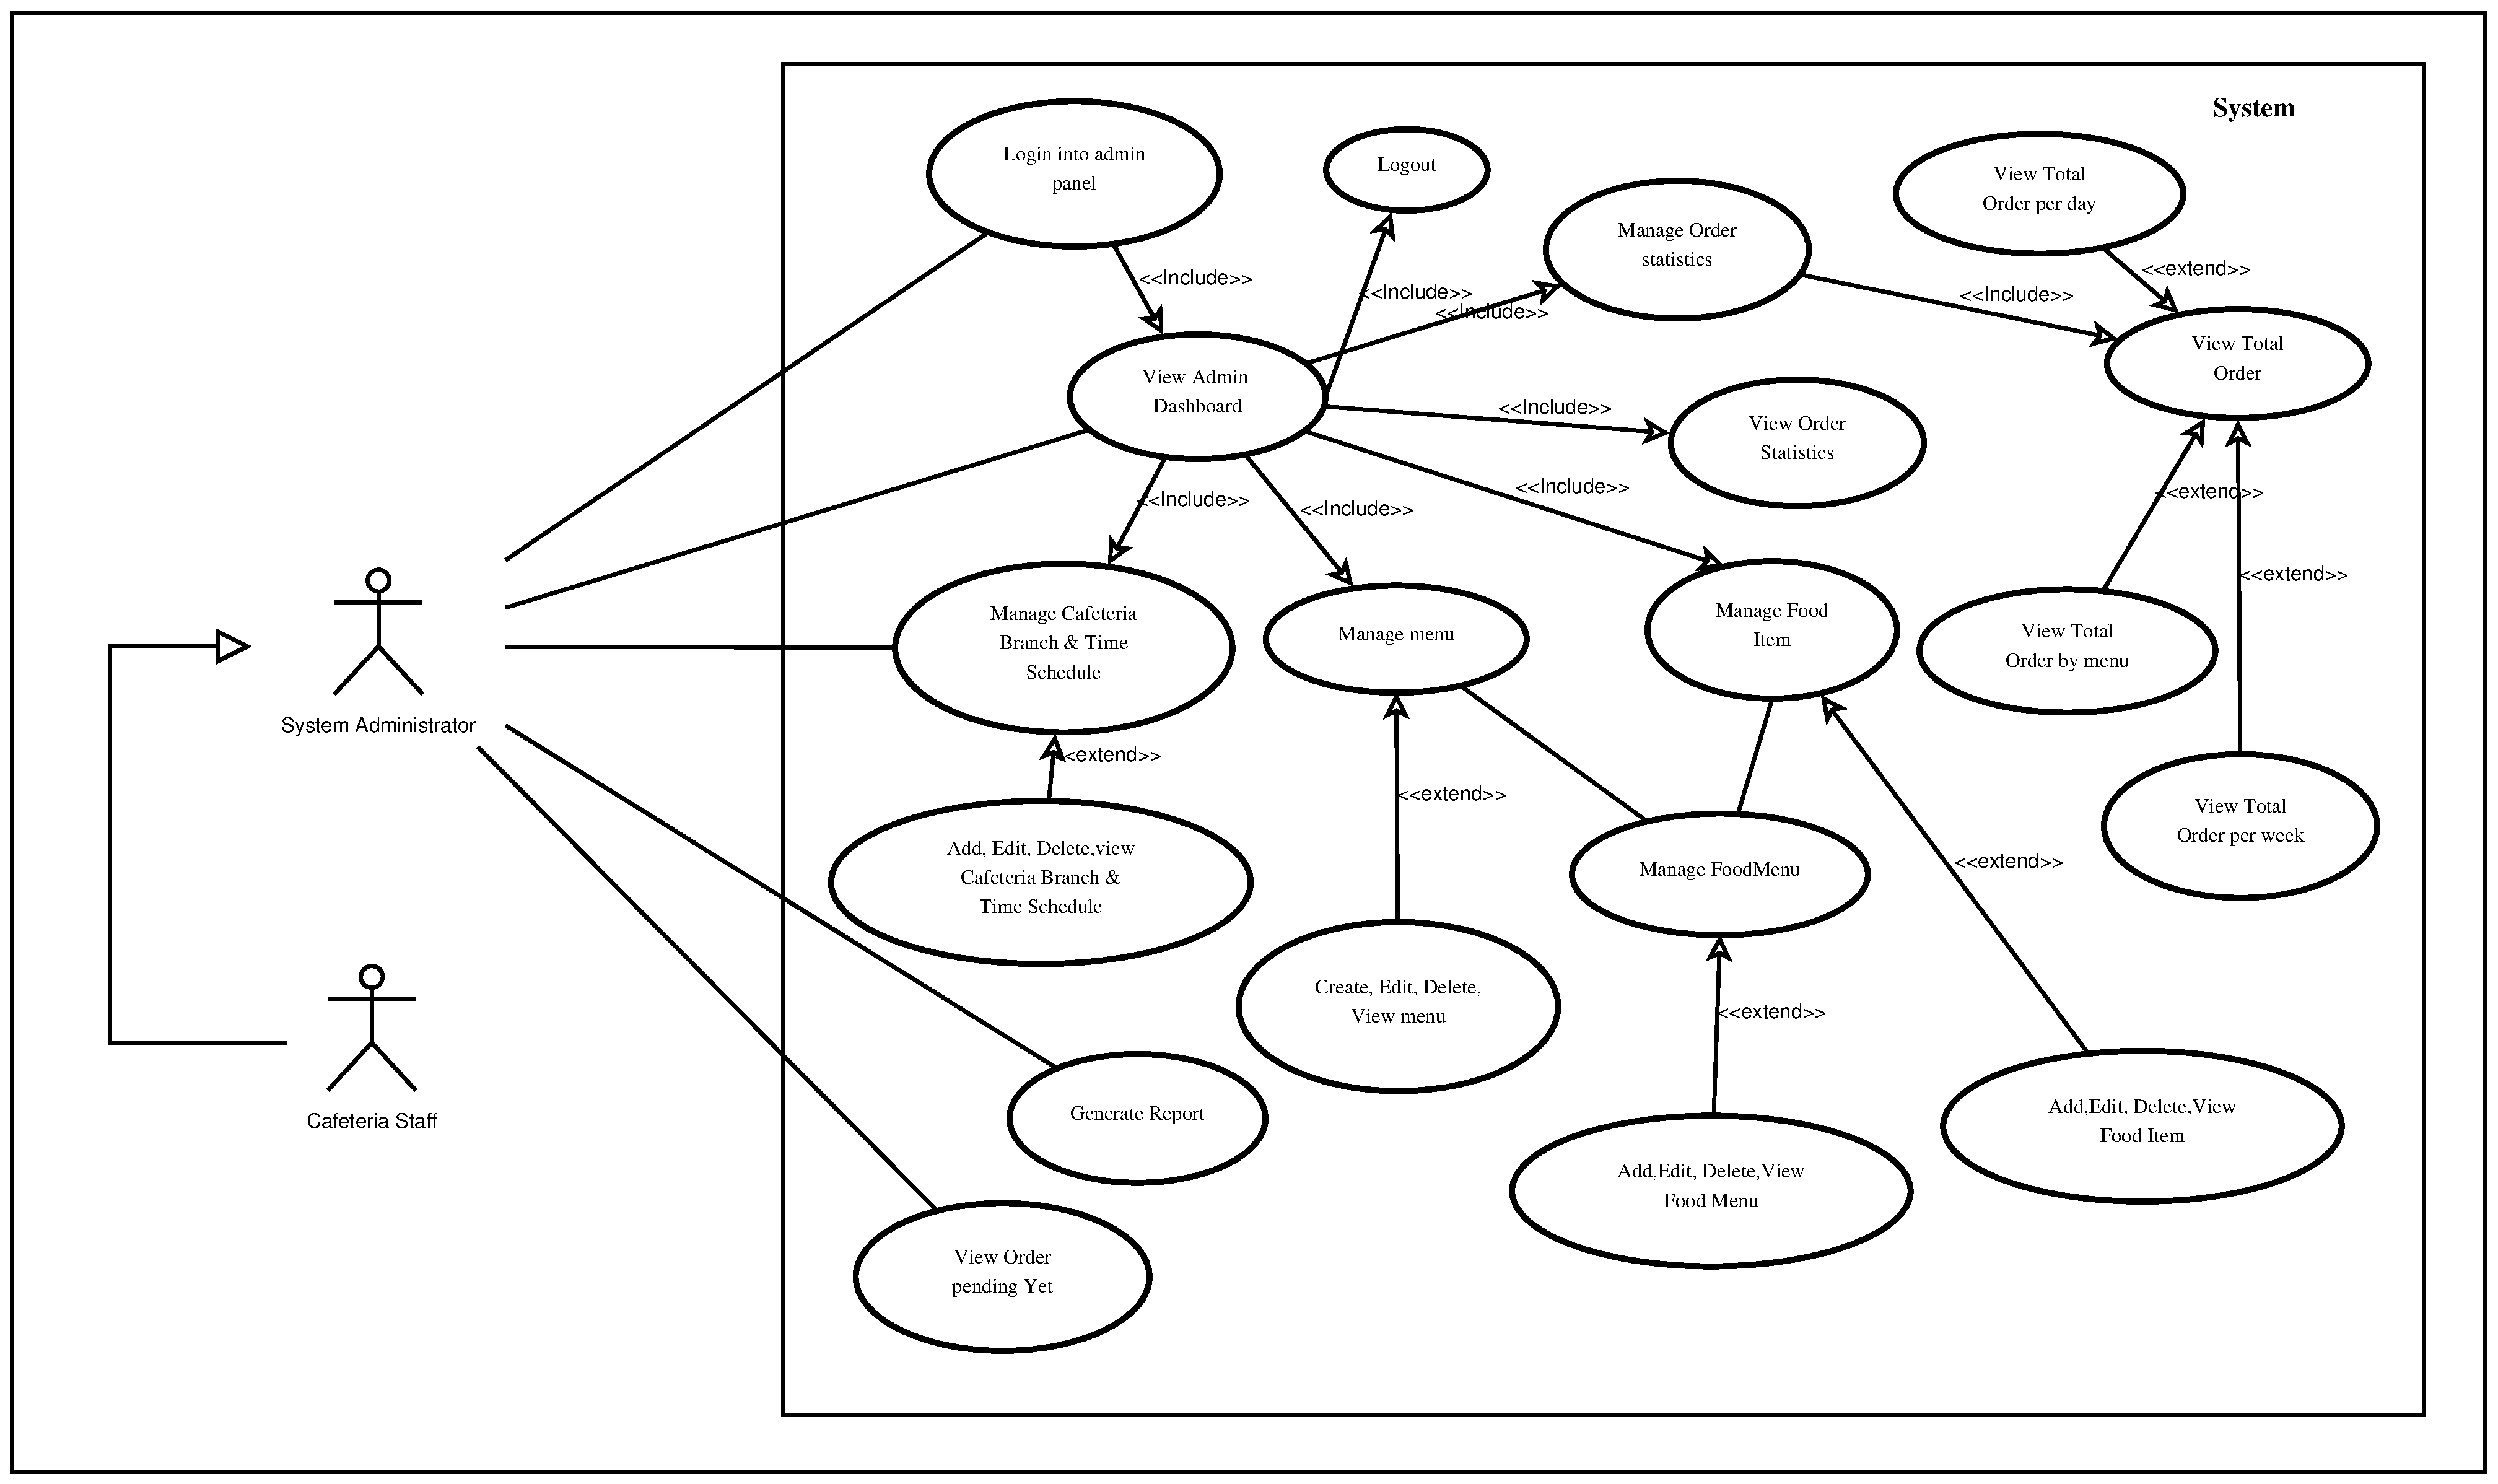
\includegraphics[width=9in]{ch3/UseCase/SystemAdministrator}
  \caption{Use Case Diagram of System Administrator}
  \label{UCSystemAdministrator}
\end{figure}
\end{landscape}

\subsubsection{Use case of System Application}

System application itself is a use case where generates various notifications
and sends to the system users either through using sms or email depends on user
preferences. System application also generates different list of food menu for
different user depending on their choices and calorie consumption of the last
couple of days. System application also make the order status pending until user
takes receipt from POS terminal  and also make the order status confirm when
user prints invoice from POS terminal punching the card.
\begin{figure}[h!t]
    \centering
      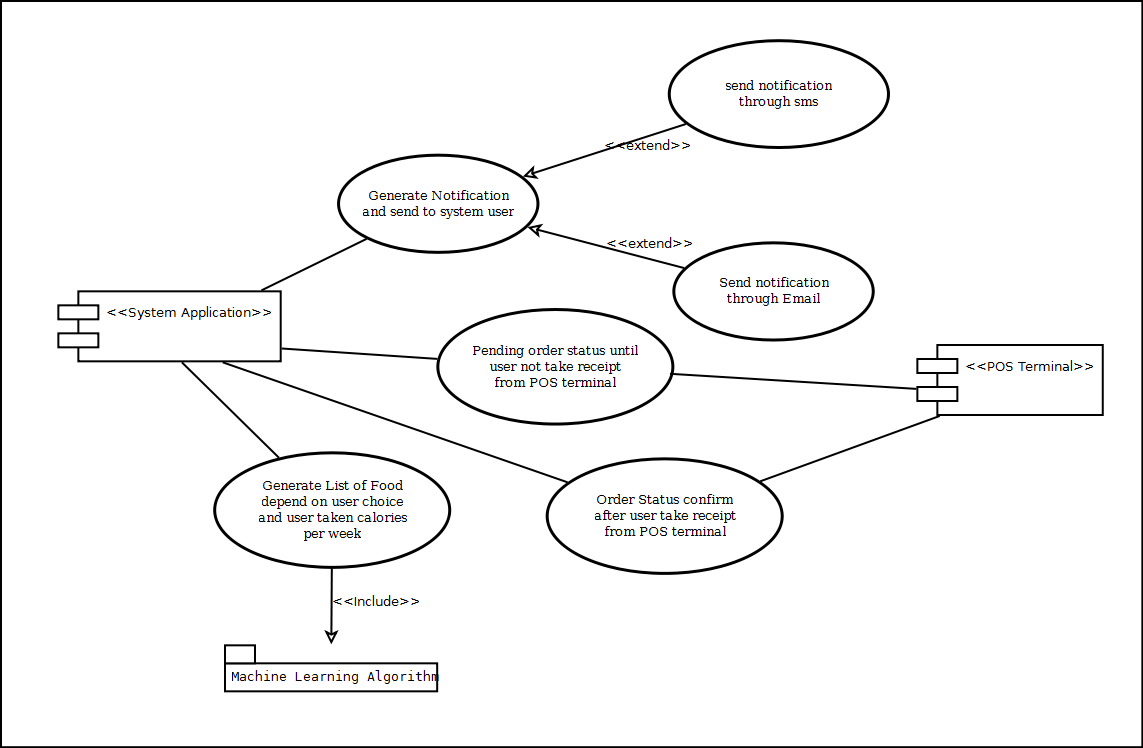
\includegraphics[width=5.5in]{ch3/UseCase/SystemApplication}
  \caption{Use Case Diagram of System Application}
  \label{UCSystemApplication}
\end{figure}

\subsubsection{Use case of POS terminal}

In the use case of POS terminal, POS terminal prints menu invoice for the system
user after he punches the card into the pos terminal after placing order for
food menu. When system user prints food menu receipt, POS terminal sends a
confirmation message to system application.
\begin{figure}[h!t]
    \centering
      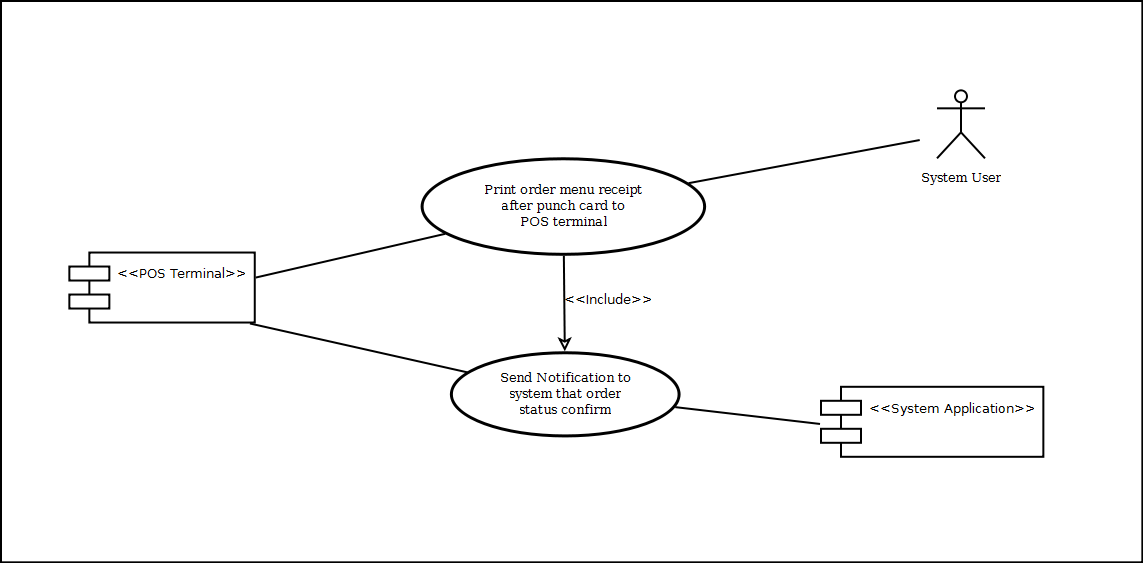
\includegraphics[width=5.5in]{ch3/UseCase/PosTerminal}
  \caption{Use Case Diagram of Pos Terminal}
  \label{UCPosTerminal}
\end{figure}
\newpage

\subsection{Class Diagram}
\label{subsec:classdiagram}
In UML 2.0 \cite{Donald} there are two basic categories of diagrams:
structure diagrams and behavior diagrams. Class diagram belongs to structure
diagrams which shows the static structure of the system which is going to be
modeled. In an object oriented application development, class diagram is very
important in initial stage to model a system. Each class consist attributes,
operations and relationships with other classes. In the following
figure~\ref{ClassDiagram}, I have modeled the class diagram of Smart cafeteria
and provided some description of each class.

\begin{landscape}
\begin{figure}[h!t]
    \centering
      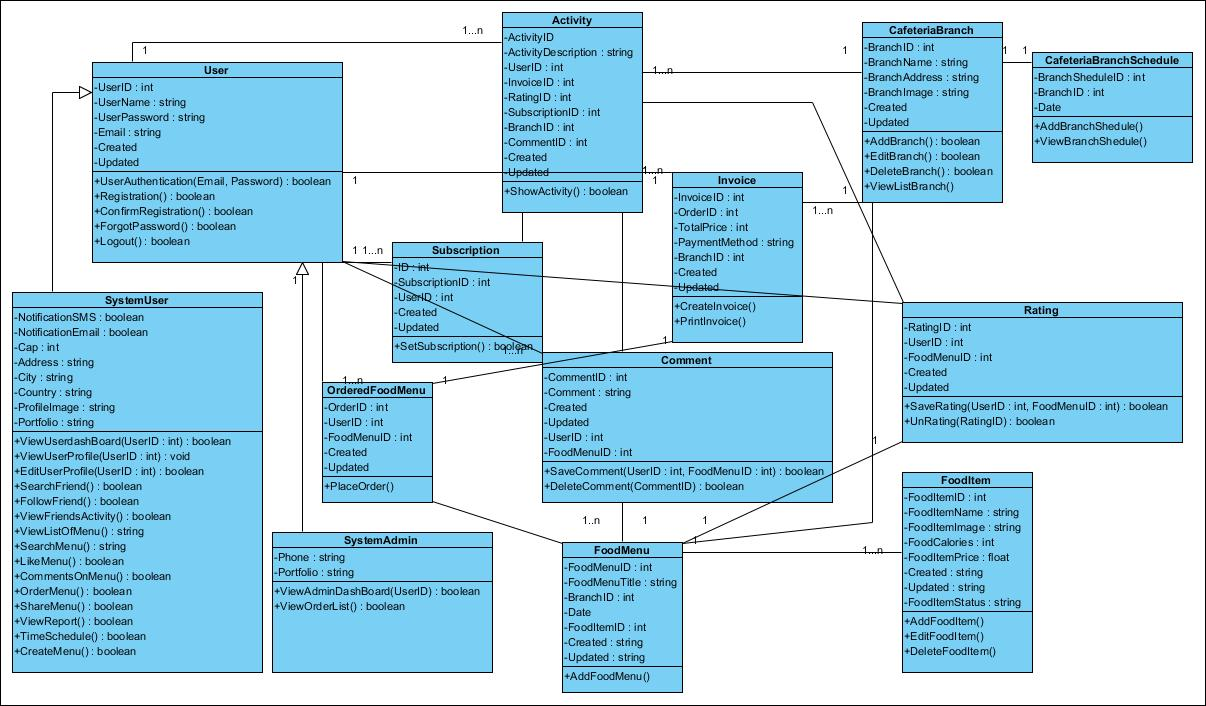
\includegraphics[width=9in]{ch3/ClassDiagram/Class}
  \caption{Class Diagram of Smart Cafeteria}
  \label{ClassDiagram}
\end{figure}
\end{landscape}
\textbf{User:} This class contains information about a user in the smart
cafeteria. The user class has a UserID as a primary key which will be unique,
UserName, UserPassword as credential information, Email address and created and
updated properties. This User class also has some functionality
UserAuthentication which will take arguments as Email and Password,
Registration, ConfirmRegistration, ForgotPassword and Logout. The user class is
associated with Activity, Subscriptions, Comments, Rating and OrderedFoodMenu
classes.

\textbf{System User:}The class System User will be inherited from User class
which means all properties and methods from User class will be included into
System User class. This class also contains some attributes such as
NotificationSMS that is a flag which gives notification users through SMS,
NotificationEmail that also gives notifications users through email, Cap,
Address, City, Country; and created and updated properties. This class also has
some functionalities such as ViewUserDashboard, ViewUserProfile,
EditUserProfile, SearchFriend, FollowFriends, Viewfriendsactivity,
ViewListofMenu, SearchMenu, Likemenu, CommentOnMenu, OrderMenu, ShareMenu,
ViewReport, TimeSchedule, CreateMenu.

\textbf{System Administrator:}The System User class also will be inherited from
User class; means all properties and methods from user class will be included
into system admin class. This class also contains some attributes such as phone
and portfolio. This class contains some functionalities such as
ViewAdminDashboard, ViewListofOrder.

\textbf{Food Item:} Food Item class has FoodItemID, FoodItemName, FoodItemImage,
FoodCalories, FoodItemPrice, FoodItemStatus, cretaed and updated attributes.
This class contains AddFoodItem, EditFoodItem and DeleteFoodtem methods. This
class is associated with FoodMenu and FoodItemID is the foreign key of FoodMenu
class.

\textbf{Food Menu:} Food Menu class contains FoodMenuID, FoodMenuTitle,
BranchID, FoodItemID, cretaed and updated properties.
This class has a method named AddFoodMenu and is associated with Comments,
Rating, FoodItem and OrderFoodMenu.

\textbf{Oder Food Menu:} The OrderedFoodMenu class contains OrderID, UserID,
FoodMenuID, cretaed and updated properties and OrderPlace function. This class
is associated with FoodMenu, Invoice and User classes.

\textbf{Invoice:} The Invoice class contains InvoiceID, OrderID, TotalPrice,
PaymentMethod, BranchID , cretaed and updated attributes. This class also has
CreateInvoice and PrintInvoice methods and associated with Activity.


\textbf{Comment:} Class Comment contains CommentID, Comment, UserID,
FoodMenuID, cretaed and updated properties and SaveComment and DeleteComment
methods. This class is associated with User and FoodMenu classes.

\textbf{Rating:} The class Rating contains RatingID, UserID, FoodMenuID,
cretaed and updated properties and SaveRating and UnRating methods. This class
is associated with User and FoodMenu classes. This class is associated with User
and FoodMenu classes.

\textbf{Subscription:} The class Subscription contains ID, SubscriptionID,
UserID, cretaed and updated properties and Subscription method. This class is
associated with User and Activity classes.

\textbf{Activity:} The class Activity has ActivityID, ActivityDescription,
UserID, InvoiceID, CommentID, RatingID, SubscriptionID, BranchID, cretaed and
updated properties and ShowActivity method. This class is associated with User,
Invoice, Comment, Rating, Subscription and Branch classes.


\textbf{CafeteriaBranch:} The class  CafeteriaBranch contains BranchID,
BranchName, BranchAddress, BranchImage, cretaed and updated properties and
AddBranch, EditBranch, DeleteBranch and ViewListBranch methods. The class
Cafeteriabranch is associated with Invoice, Activity and CafeteriaBranchShedule
classes.

\textbf{CafeteriaBranchSchedule:} The class CafeteiraBranchSchedule contains
BranchScheduleID, BranchID and Date properties and AddBranchSchedule,
ViewBranchSchedule methods. This class is associated with CafeteriaBranch class.


\subsection{Activity Diagram}
\label{subsec:activity}
Activity diagram \cite{UMLActivityDiagram} describes dynamic aspects of any system and
basically represents the flow of activity form one to another activity. The
activity could be described as an operation of the system and this diagram
captures the dynamic behavior of the system. So it is important to visualize
dynamic nature of a system. In this analysis, I have found some activity diagram
of Smart Cafeteria system and shown in figure[\ref{SystemUserActivityDiagram},
\ref{AdministratorActivityDiagram}, \ref{SystemActivityDiagram},
\ref{PointofSaleActivity}] and described step by step.

\subsubsection{System User} When a user browses the system, he or she can
navigate to search food menu, see time schedule, see today's top menu into the
slideshow and browse today's food menus. Users also can register in the system
and login into the system.  After successfully login into the system, user as a
registered user could navigate previous basic activities search food menu, see
time schedule as well as could browse User Dashboard from where user could
search friends, follow friends, see friend's activities, see dieting reports,
create food menu from foods, comment on food menus, like food menus, share food
menus and order food menus. Users also could change profiles and logout from
this stage.
The system will do some activities alone with user such as suggest daily
different food menus for different users based on users interest and previous
food consumed and dieting history. System will also save registration
information of user after registration and check account credential before login
action. After all actions, system saves preferences as well. In the figure
\ref{SystemUserActivityDiagram}, shows the activity of users as simultaneously
with system.

\begin{landscape}
\begin{figure}[h!t]
    \centering
      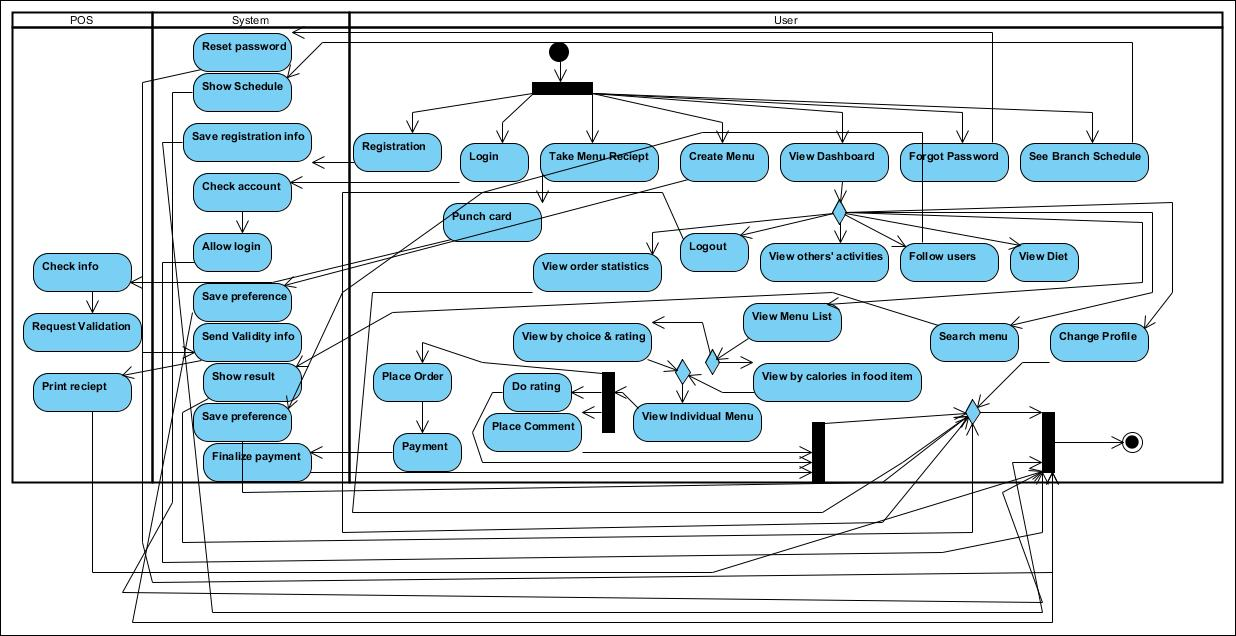
\includegraphics[width=8in,height=5in]{ch3/ActivityDiagram/SystemUser}
  \caption{System User Activity Diagram of Smart Cafeteria}
  \label{SystemUserActivityDiagram}
\end{figure}
\end{landscape}

\subsubsection{System Administrator} System administrator has some flow of activity
after login into the system using administrator panel. System Administrator
could view order pending from user's order and can confirm the order; and
search report and system show report as well. From dashboard, system
administrator can do different activity; manage food item, food menu, view order
statistics and manage order statistics into different request such as view order
by day, view order by month or view order by menu; and system response as well
in the every activity.In the figure \ref{AdministratorActivityDiagram}, shows
the activity of System Administrator.

\begin{figure}[h!t]
    \centering
      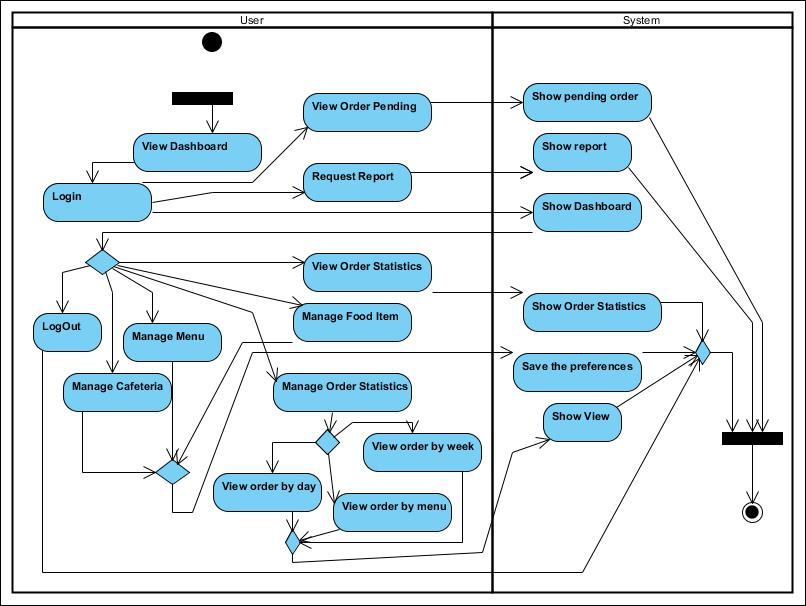
\includegraphics[width=5.5in]{ch3/ActivityDiagram/SysAdmin}
  \caption{System Administrator Activity Diagram}
  \label{AdministratorActivityDiagram}
\end{figure}

\subsubsection{System} In the system, there are some very important activities such
as receive order confirmation from users, generate diet reports, create food
suggestions, generate different kinds of notifications and send to users. The
system looks after both type of user's; system users and system administrators,
session and credentials as well. In the figure \ref{SystemActivityDiagram} shows
the activity of System.
\begin{figure}[h!t]
    \centering
      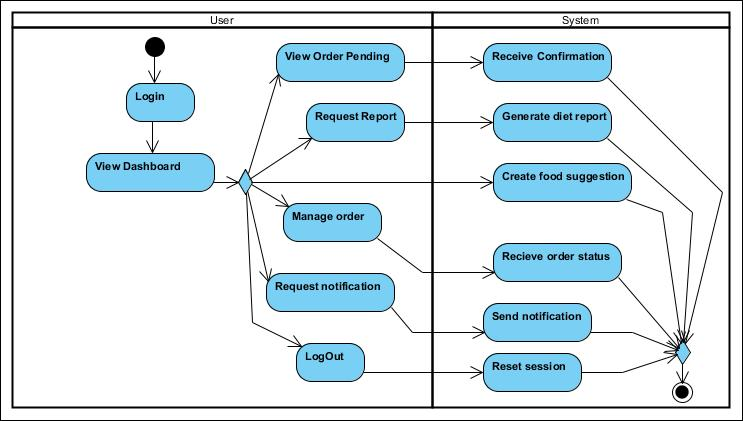
\includegraphics[width=5.5in]{ch3/ActivityDiagram/SysApp}
  \caption{System Activity Diagram}
  \label{SystemActivityDiagram}
\end{figure}

\subsubsection{Point of Sale} After confirmation of order, users punch card into
POS terminal and those POS terminations are responsible to print order receipt
for users and send a notification to the system application to update that the
food menu is being served. In the figure \ref{PointofSaleActivity} shows the
activity of Point of Sale.

\begin{figure}[h!t]
    \centering
      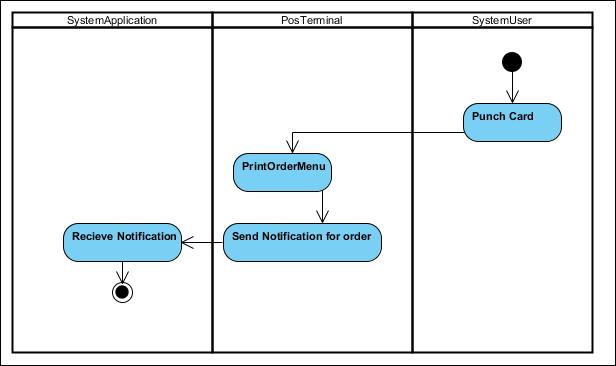
\includegraphics[width=5.5in]{ch3/ActivityDiagram/POS}
  \caption{Point of Sale Activity Diagram}
  \label{PointofSaleActivity}
\end{figure}